% Frame data sources M1
\begin{frame}{\textbf{Data sources}}
    \begin{itemize}
      \item \textbf{Real-time pings}: real-time data on vehicle number, date and time, latitude, longitude, driver identification number (ID), and speed. Collected every 1 to 10 minutes.
      \item \textbf{safety critical events, SCEs}: 1) hard brake (HB), 2) headway (HW), 3) collision mitigation (CM), and 4) rolling stability (RS).
      \item \textbf{Driver demographics}: driver \textit{age}.
      \item \textbf{Road geometry}: \textit{speed limits} and \textit{the number of lanes} from the OpenStreetMap API.
      \item \textbf{Weather}: \textit{precipitation intensity}, \textit{precipitation probability}, \textit{wind speed}, and \textit{visibility}, from the Dark Sky API.
  \end{itemize}
\end{frame}

% Frame data transformation M2
\begin{frame}{\textbf{Data transformation}}
    \begin{itemize}
      \item \textbf{Trips}:  real-time ping stopped for $\geq20$ minutes, the ping data will be separated into two different trips. A trip is \textit{short continuous driving intervals} with a mean length of 1.8 hours.
      \item \textbf{Half-hour intervals}: trip length is heterogeneous (5 minutes to $\geq8$ hours),  so trips were further divided into half-an-hour fixed intervals.
      \item \textbf{Shifts}: the trips will be further divided into different shifts if the driver was not moving for at least eight hours. A shift is therefore a long driving time with \textit{intermittent short rests} (20 minutes to $<8$ hours).
      \item \textbf{A proxy of driver fatigue}: cumulative summation of interval time within a shift for each driver as the \textit{cumulative driving time}.
  \end{itemize}
\end{frame}

% Frame data merging (flow chart) M3
\begin{frame}{\textbf{Data merging}}
\centering
  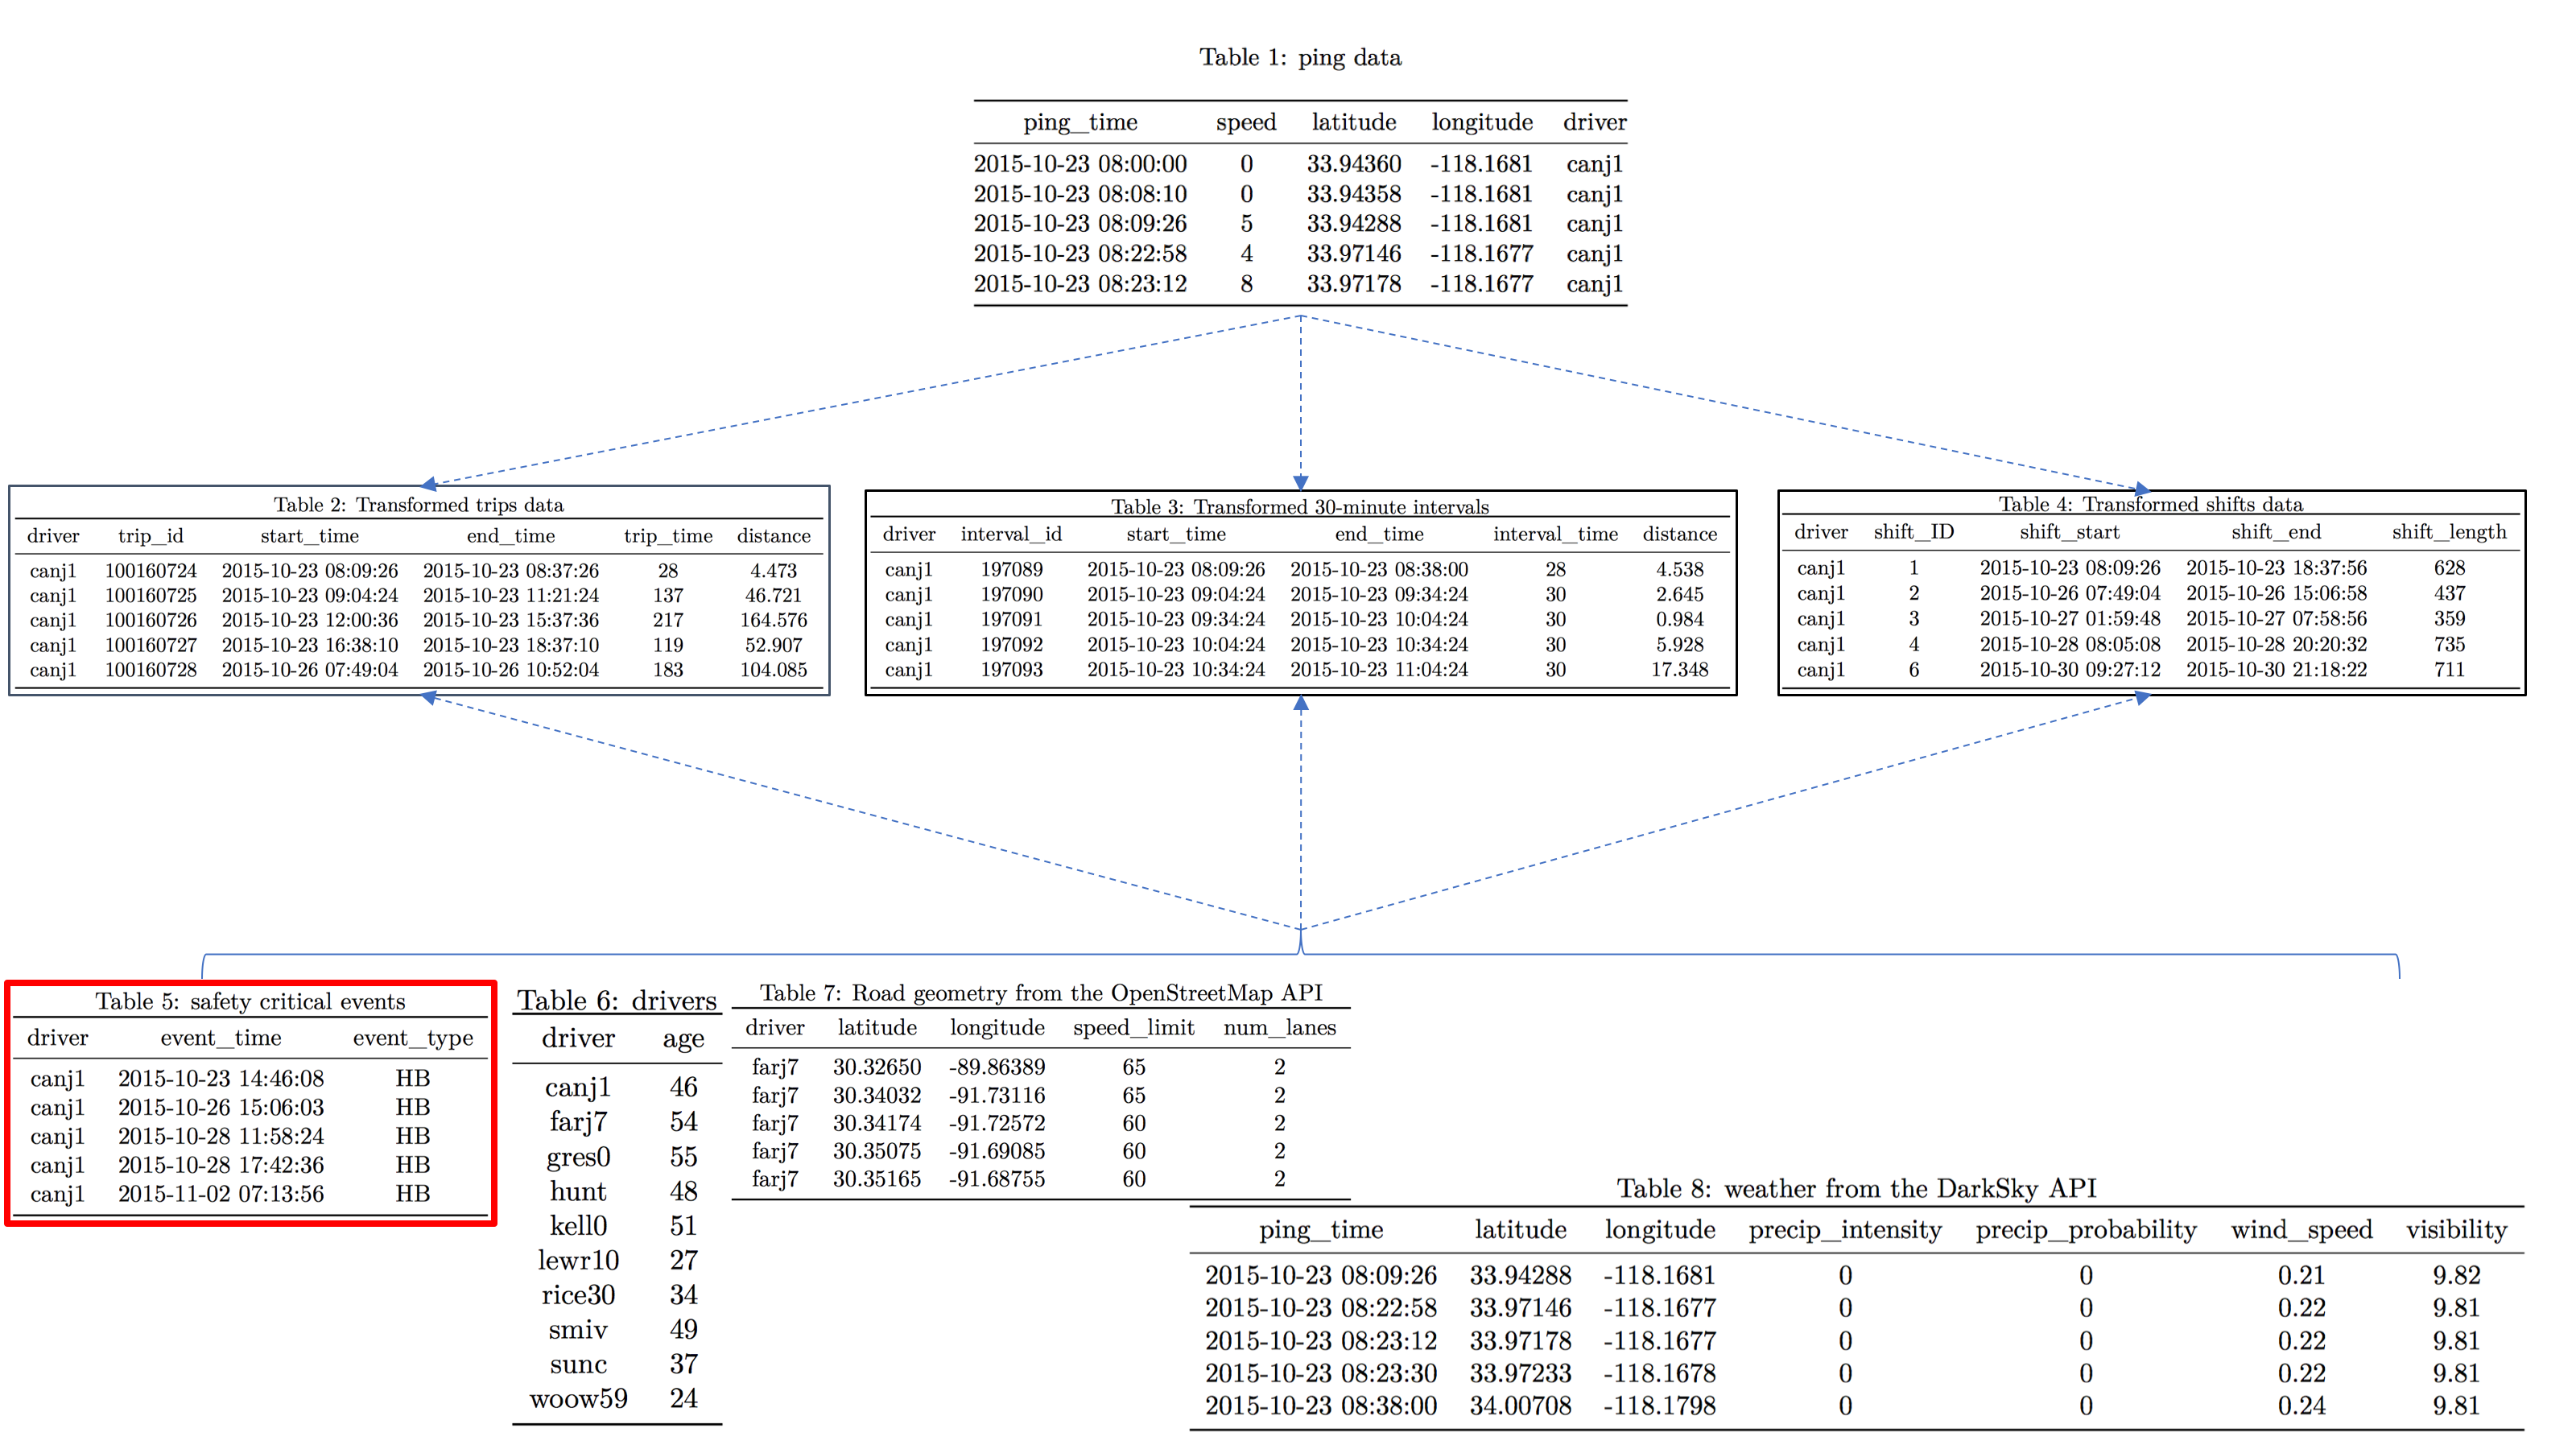
\includegraphics[width=\textwidth, height = \textheight, keepaspectratio, frame]{Figures/flow_chart.png}
\end{frame}

% Frame logit
\begin{frame}{\textbf{Bayesian random-effects logistic regression}}
\begin{equation}\label{eq:logit}
\begin{split}
Y_{i} &\sim \text{Bernoulli}(p_{i})\\
\log\frac{p_{i}}{1-p_{i}} &= \beta_{0, d(i)} + \beta_{1, d(i)} \cdot \text{CT}_i + \sum_{j=1}^{J} x_{ij}\beta_j\\
\beta_{0, d} &\sim \text{i.i.d. } N(\mu_0, \sigma_0^2), \quad d = 1, 2, \cdots, D\\
\beta_{1, d} &\sim \text{i.i.d. } N(\mu_1, \sigma_1^2), \quad d = 1, 2, \cdots, D
\end{split}
\end{equation}
\begin{itemize}
    \item $Y_i$: whether SCEs occurred during the interval, 0 or 1,
    \item CT$_i$: cumulative driving time,
    \item $\beta_{0, d}$: random intercepts for each driver,
    \item $\beta_{1, d}$: random slopes for CT$_i$ for each driver,
    \item $x_{ij}$: covariates, including age, road geometry, and weather.
\end{itemize}
\end{frame}

% Frame Poisson
\begin{frame}{\textbf{Bayesian random-effects Poisson regression}}
\begin{equation}\label{eq:pois}
\begin{split}
Y_{i}  & \sim \text{Poisson}(T_i\cdot\lambda_i)\\
\log\lambda_{i} & =\beta_{0, d(i)} + \beta_{1, d(i)} \cdot \text{CT}_i + \sum_{j=1}^{J} x_{ij}\beta_j\\
\beta_{0, d} &\sim \text{i.i.d. } N(\mu_0, \sigma_0^2), \quad d = 1, 2, \cdots, D\\
\beta_{1, d} &\sim \text{i.i.d. } N(\mu_1, \sigma_1^2), \quad d = 1, 2, \cdots, D
\end{split}
\end{equation}
\begin{itemize}
    \item $Y_i$: the number of SCEs during the interval, a non-negative integer,
    \item $T_i$: length of the interval as an offset term,
    \item CT$_i$: cumulative driving time,
    \item $\beta_{0, d}$: random intercepts for each driver,
    \item $\beta_{1, d}$: random slopes for CT$_i$ for each driver,
    \item $x_{ij}$: covariates, including age, road geometry, and weather.
\end{itemize}
\end{frame}

% Frame priors
\begin{frame}
\textbf{Weakly informative} priors and hyper-priors as recommended by Gelman \cite{gelman2017prior}.
\begin{equation}
	\label{eq:prior}
	\begin{split}
		\mu_0 & \sim N(0, 5^2)\\
		\mu_1 & \sim N(0, 5^2)\\
		\sigma_0 & \sim \text{Gamma}(1, 1)\\
		\sigma_1 & \sim \text{Gamma}(1, 1)\\
		\beta_2, \beta_3, \cdots, \beta_J  & \sim N(0, 10^2)
	\end{split}
\end{equation}
\begin{itemize}
    \item $\mu_0, \sigma_0$: hyper-parameters for $\beta_{0, d}$,
    \item $\mu_1, \sigma_1$: hyper-parameters for $\beta_{1, d}$,
    \item $\beta_2, \beta_3, \cdots, \beta_J$: fixed parameters for covariates $x_{ij}$.
\end{itemize}
\end{frame}

% Frame NHPP - theory
\begin{frame}{\textbf{Non-homogeneous Poisson process: introduction}}
\begin{itemize}
    \item The \textbf{intensity function} of a point process is $$\lambda(t) = \lim_{\Delta t \rightarrow 0}\frac{P(N(t, t+\Delta t] \geq 1)}{\Delta t}$$
    \item \textbf{Nonhomogeneous Poisson Process (NHPP)}: a Poisson process whose intensity function is non-constant.
    \item \textbf{Power law process (PLP)}: the intensity function of a NHPP is $$\lambda(t) = \frac{\beta}{\theta}\bigg(\frac{t}{\theta}\bigg)^{\beta-1}, \quad \beta > 0, \theta > 0.$$
    \item $\beta$ is the shape parameter.  $\theta$ is the scale parameter.
    \item $\beta > 1 \rightarrow$ reliability deterioration; $\beta > 1 \rightarrow$ reliability improvement.
\end{itemize}
\end{frame}

% Frame NHPP - notations
\begin{frame}{\textbf{Non-homogeneous Poisson process: data}}
\begin{columns}
\begin{column}{.64\textwidth}
\begin{itemize}
\item $T_{d, s, i}$: the time to the $d$-th driver's $s$-th shift's $i$-th critical event,
\item $d$: driver index, $d = 1, 2, \cdots, D$
\item $s$: shift index, $s = 1, 2, \cdots, S_d$,
\item $i$: SCE index, $i = 1, 2, \cdots, n_{d, S_d}$
\item $n_{d,s}$: the total number critical events of $d$-th driver's $s$-th shift. 
\end{itemize}
\end{column}
\hfill
\begin{column}{.35\textwidth}
\begin{figure}
  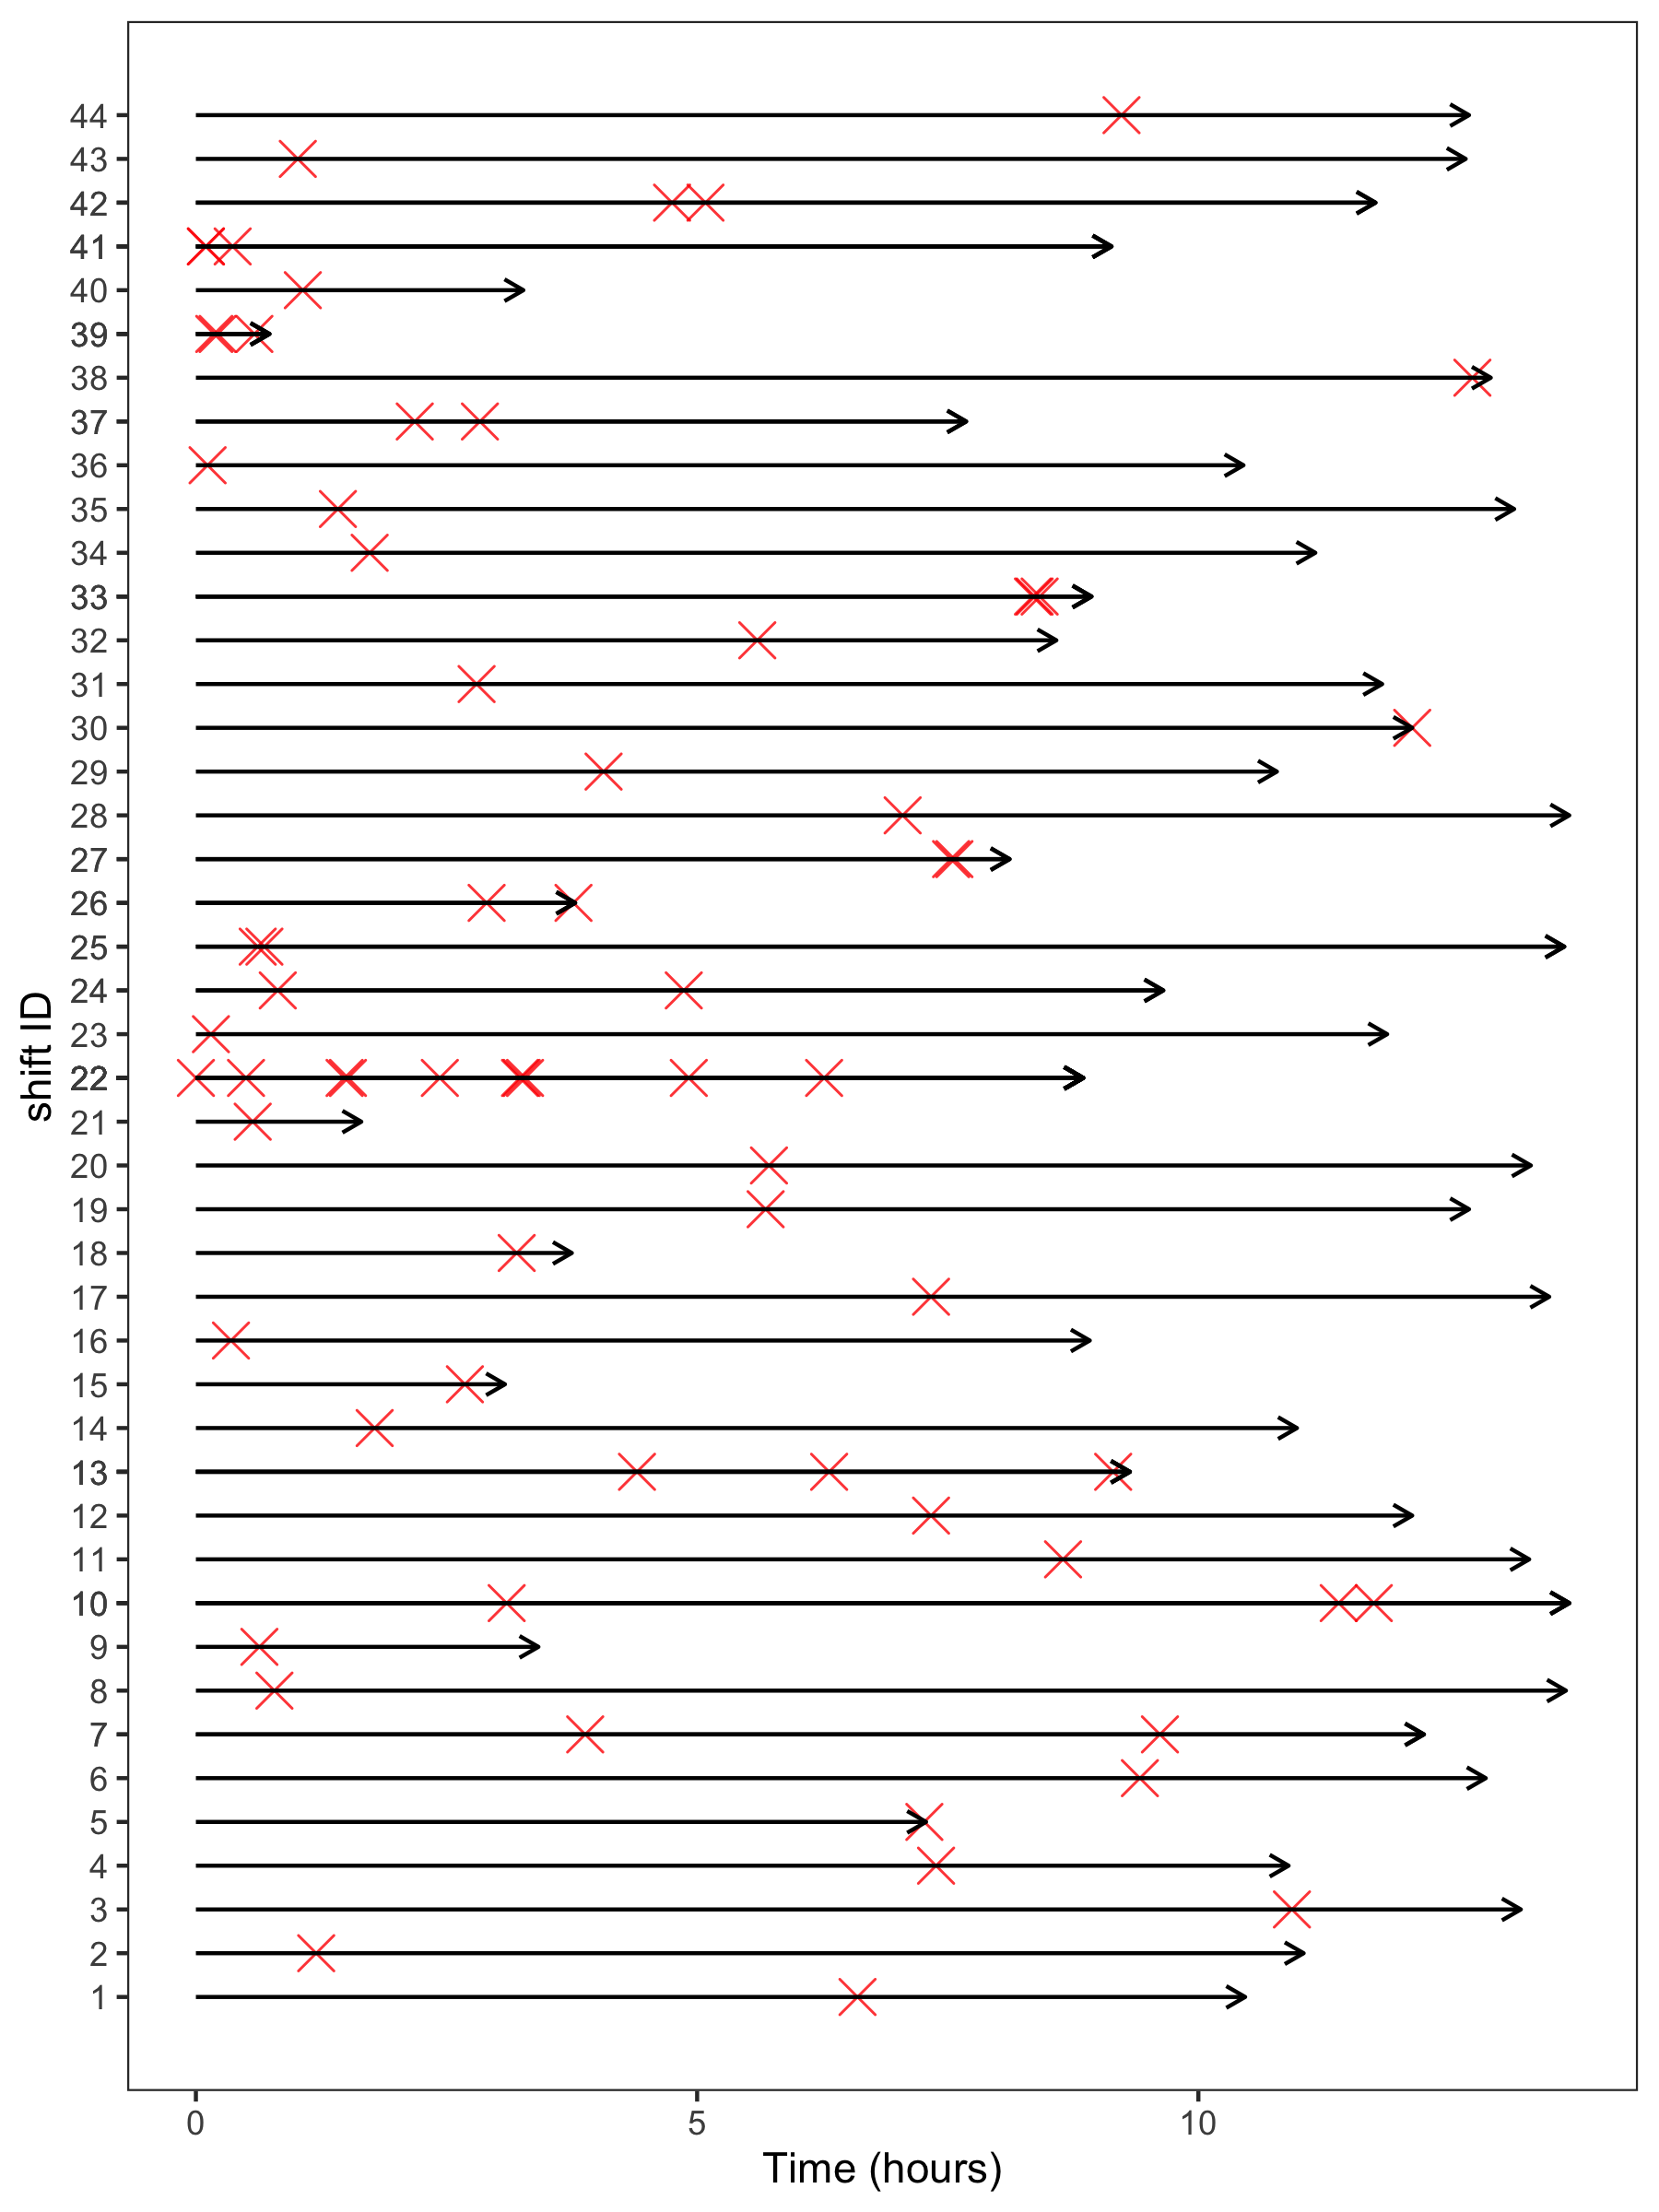
\includegraphics[width=\textwidth]{Figures/t2events_arrow_plot.png}
  \caption{Arrow plot of time to SCEs in each shift}
\end{figure}
\end{column}
\end{columns}
\end{frame}

% Frame NHPP - stats model
\begin{frame}{\textbf{Bayesian random-intercepts NHPP}}
\begin{equation}\label{eq:nhpp}
\begin{aligned}
T_{d, s, 1}, T_{d, s, 2}, \cdots , T_{d, s, n_{d, s}} & \sim \text{PLP}(\beta, \theta_{d, s})\\
\beta & \sim \text{Gamma}(1, 1)\\
\log\theta_{d, s} &= \gamma_{0d} + \gamma_{1}x_{d, s, 1} + \gamma_{2}x_{d, s, 2} + \cdots + \gamma_{k}x_{d, s, k}\\
\gamma_{01}, \gamma_{02}, \cdots, \gamma_{0D} & \sim \text{i.i.d. }N(\mu_0, \sigma_0^2)\\
\gamma_1, \gamma_2, \cdots, \gamma_k & \sim \text{i.i.d. }N(0, 10^2)\\
\mu_0 &\sim N(0, 5^2) \\
\sigma_0 &\sim \text{Gamma}(1, 1)
\end{aligned}
\end{equation}
\begin{itemize}
    \item a fixed $\beta$ across drivers, 
    \item random parameters $\theta_{d, s}$ across drivers
    \item $\theta_{d, s}$: random intercepts $\gamma_{0d}$ for scale parameter $\theta$,
    \item $x_{d, s, k}$: covariates.
\end{itemize}
\end{frame}

% Frame - Bayesian estimation
\begin{frame}{\textbf{Bayesian estimation with rstan}}
\begin{columns}
\begin{column}{.65\textwidth}
\begin{itemize}
    \item Hamiltonian Monte Carlo with No-U-Turn sampler \cite{hoffman2014no, carpenter2017stan},
    \item 4 chains, 1,000 warm-ups, 2000 iterations,
    \item Convergence diagnostics:
    \begin{itemize}
        \item Gelman-Rubin statistics $\hat{R} < 1.1$ \cite{gelman1992inference},
        \item Effective sample size (ESS) $> 500$,
        \item No divergent transitions after warmup,
        \item Traceplots.
    \end{itemize}
    \item All data and code available at \href{https://github.com/caimiao0714/ISQC2019truck}{https://github.com/caimiao0714/ISQC2019truck}.
\end{itemize}
\end{column}
\hfill
\begin{column}{.35\textwidth}
\begin{figure}
  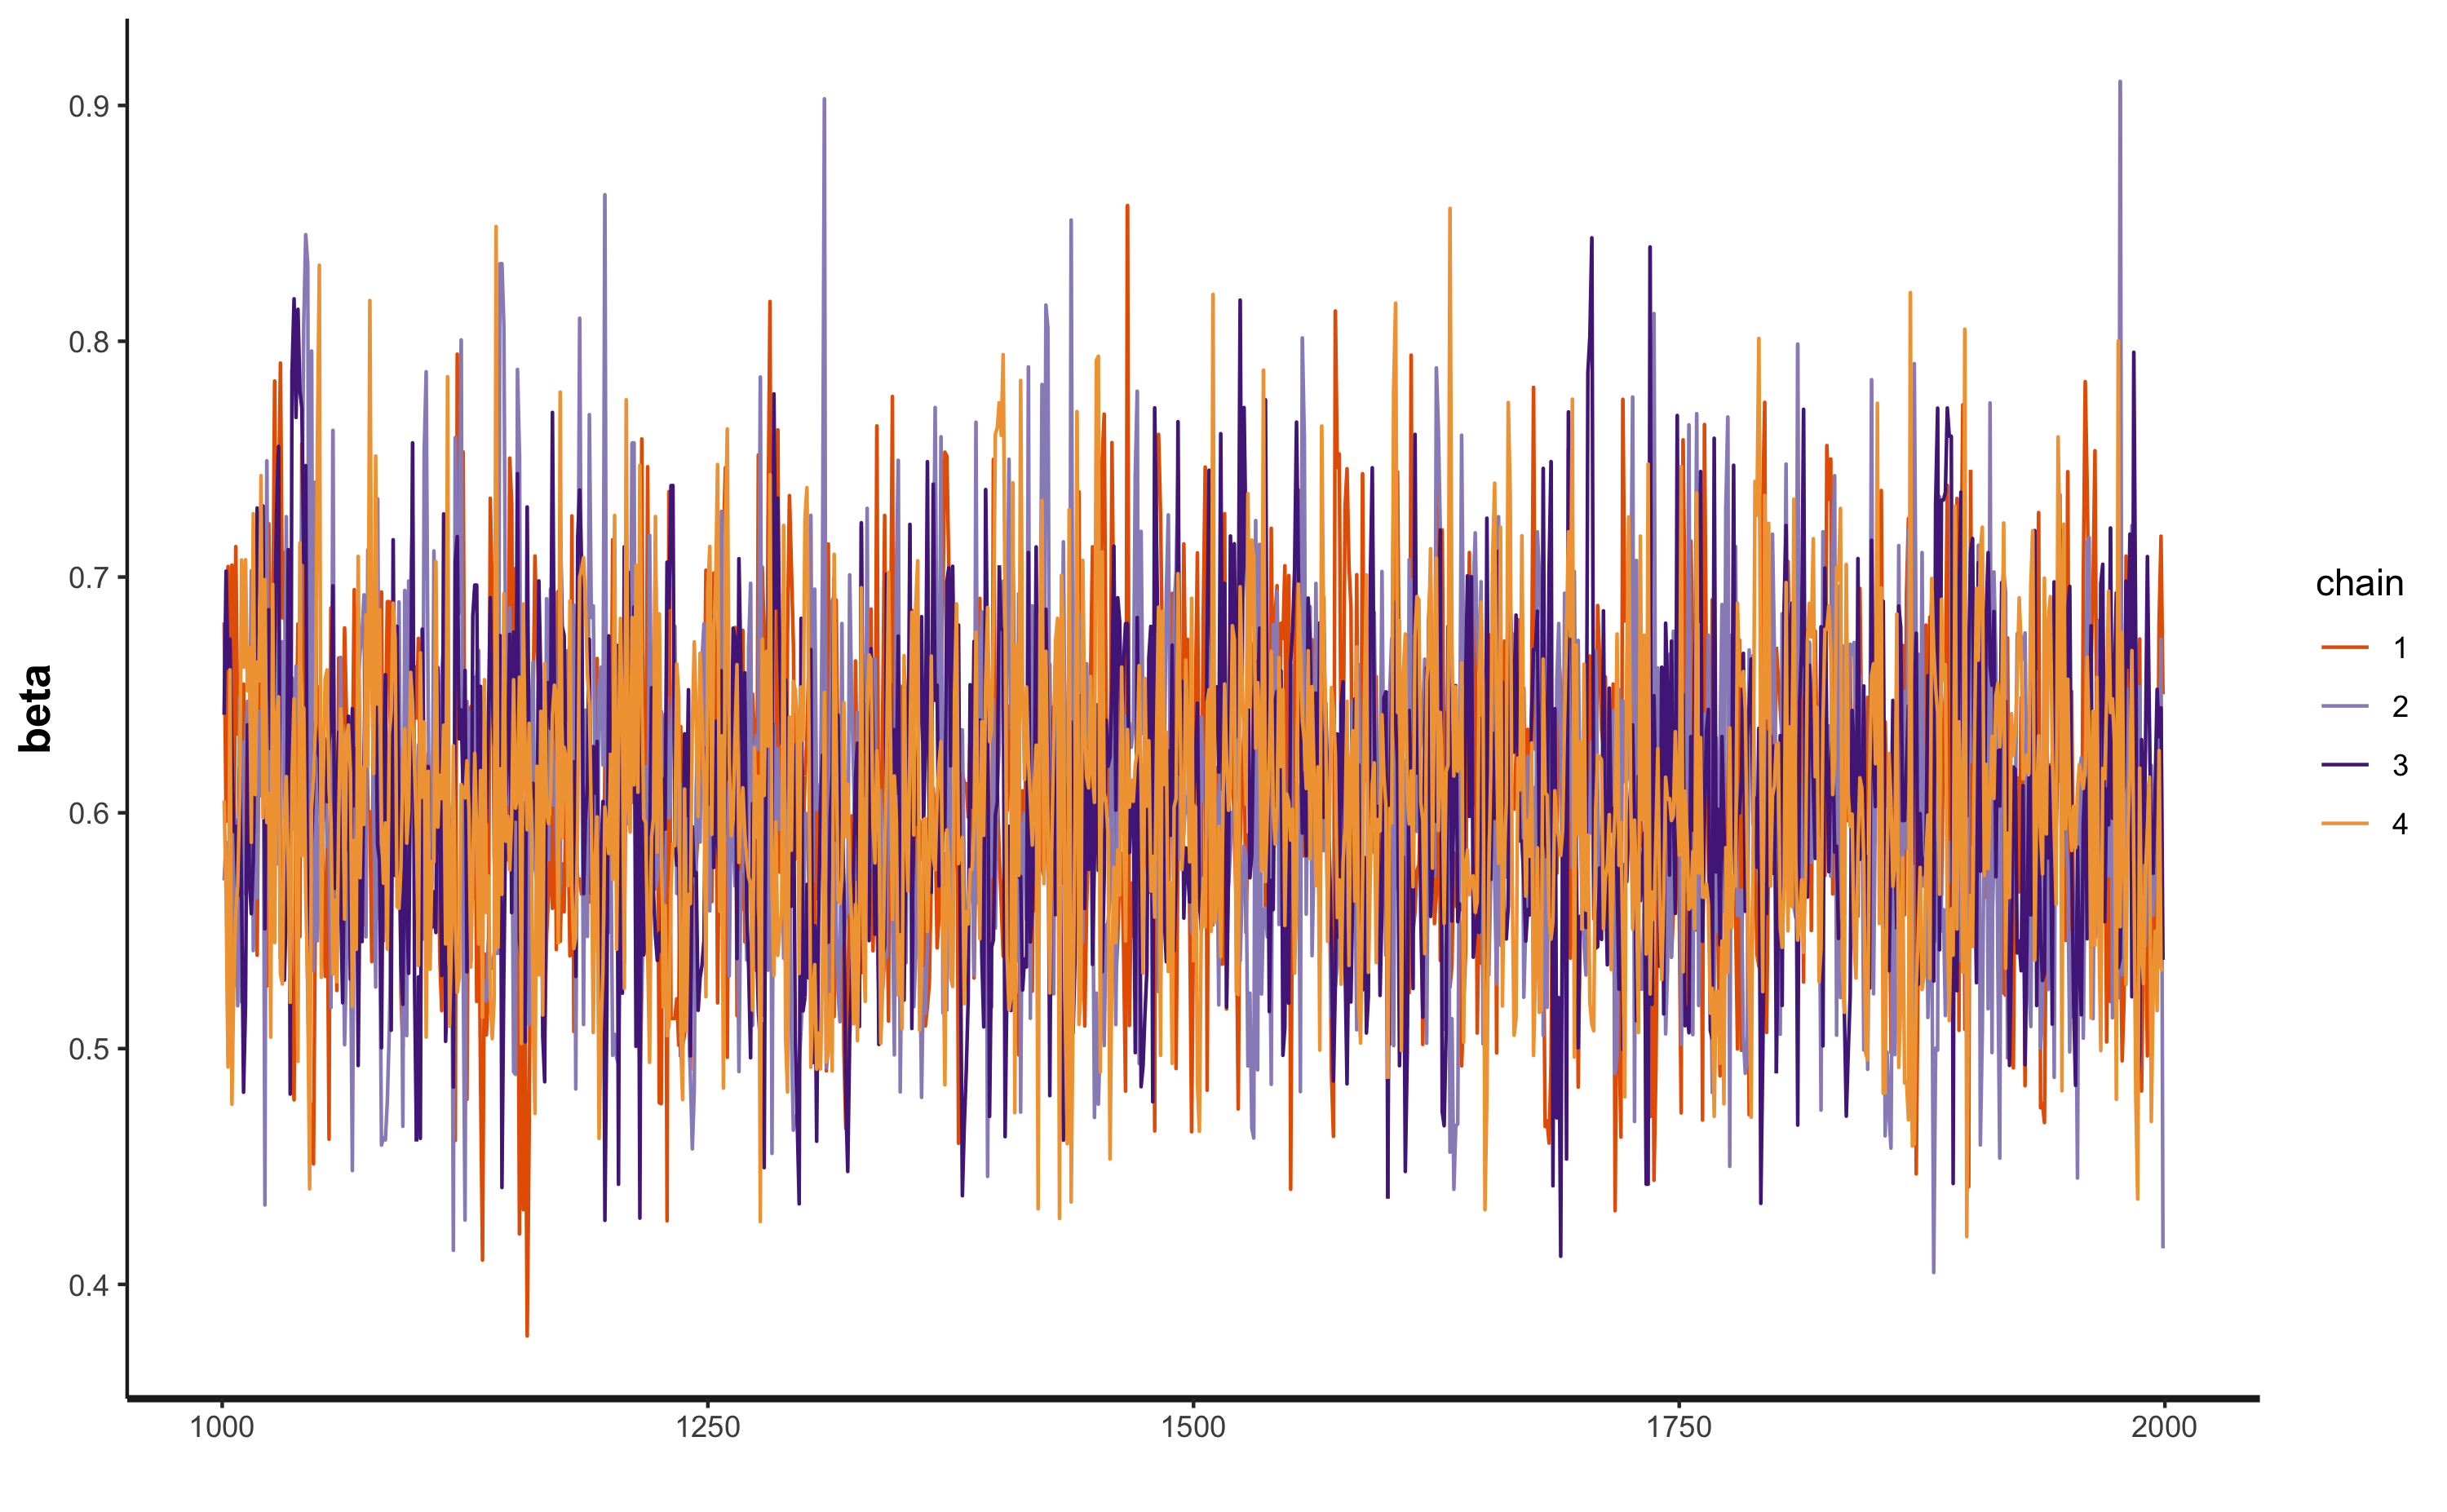
\includegraphics[width=\textwidth]{Figures/traceplot_beta.png}
  \caption{Example trace plot for the shape parameter in NHPP}
\end{figure}
\end{column}
\end{columns}
\end{frame}

% Frame - results: logit and Poisson
\begin{frame}{\textbf{Results for hierarchical Bayesian logit and Poisson regressions}}
\begin{columns}
\begin{column}{.45\textwidth}
\begin{figure}
  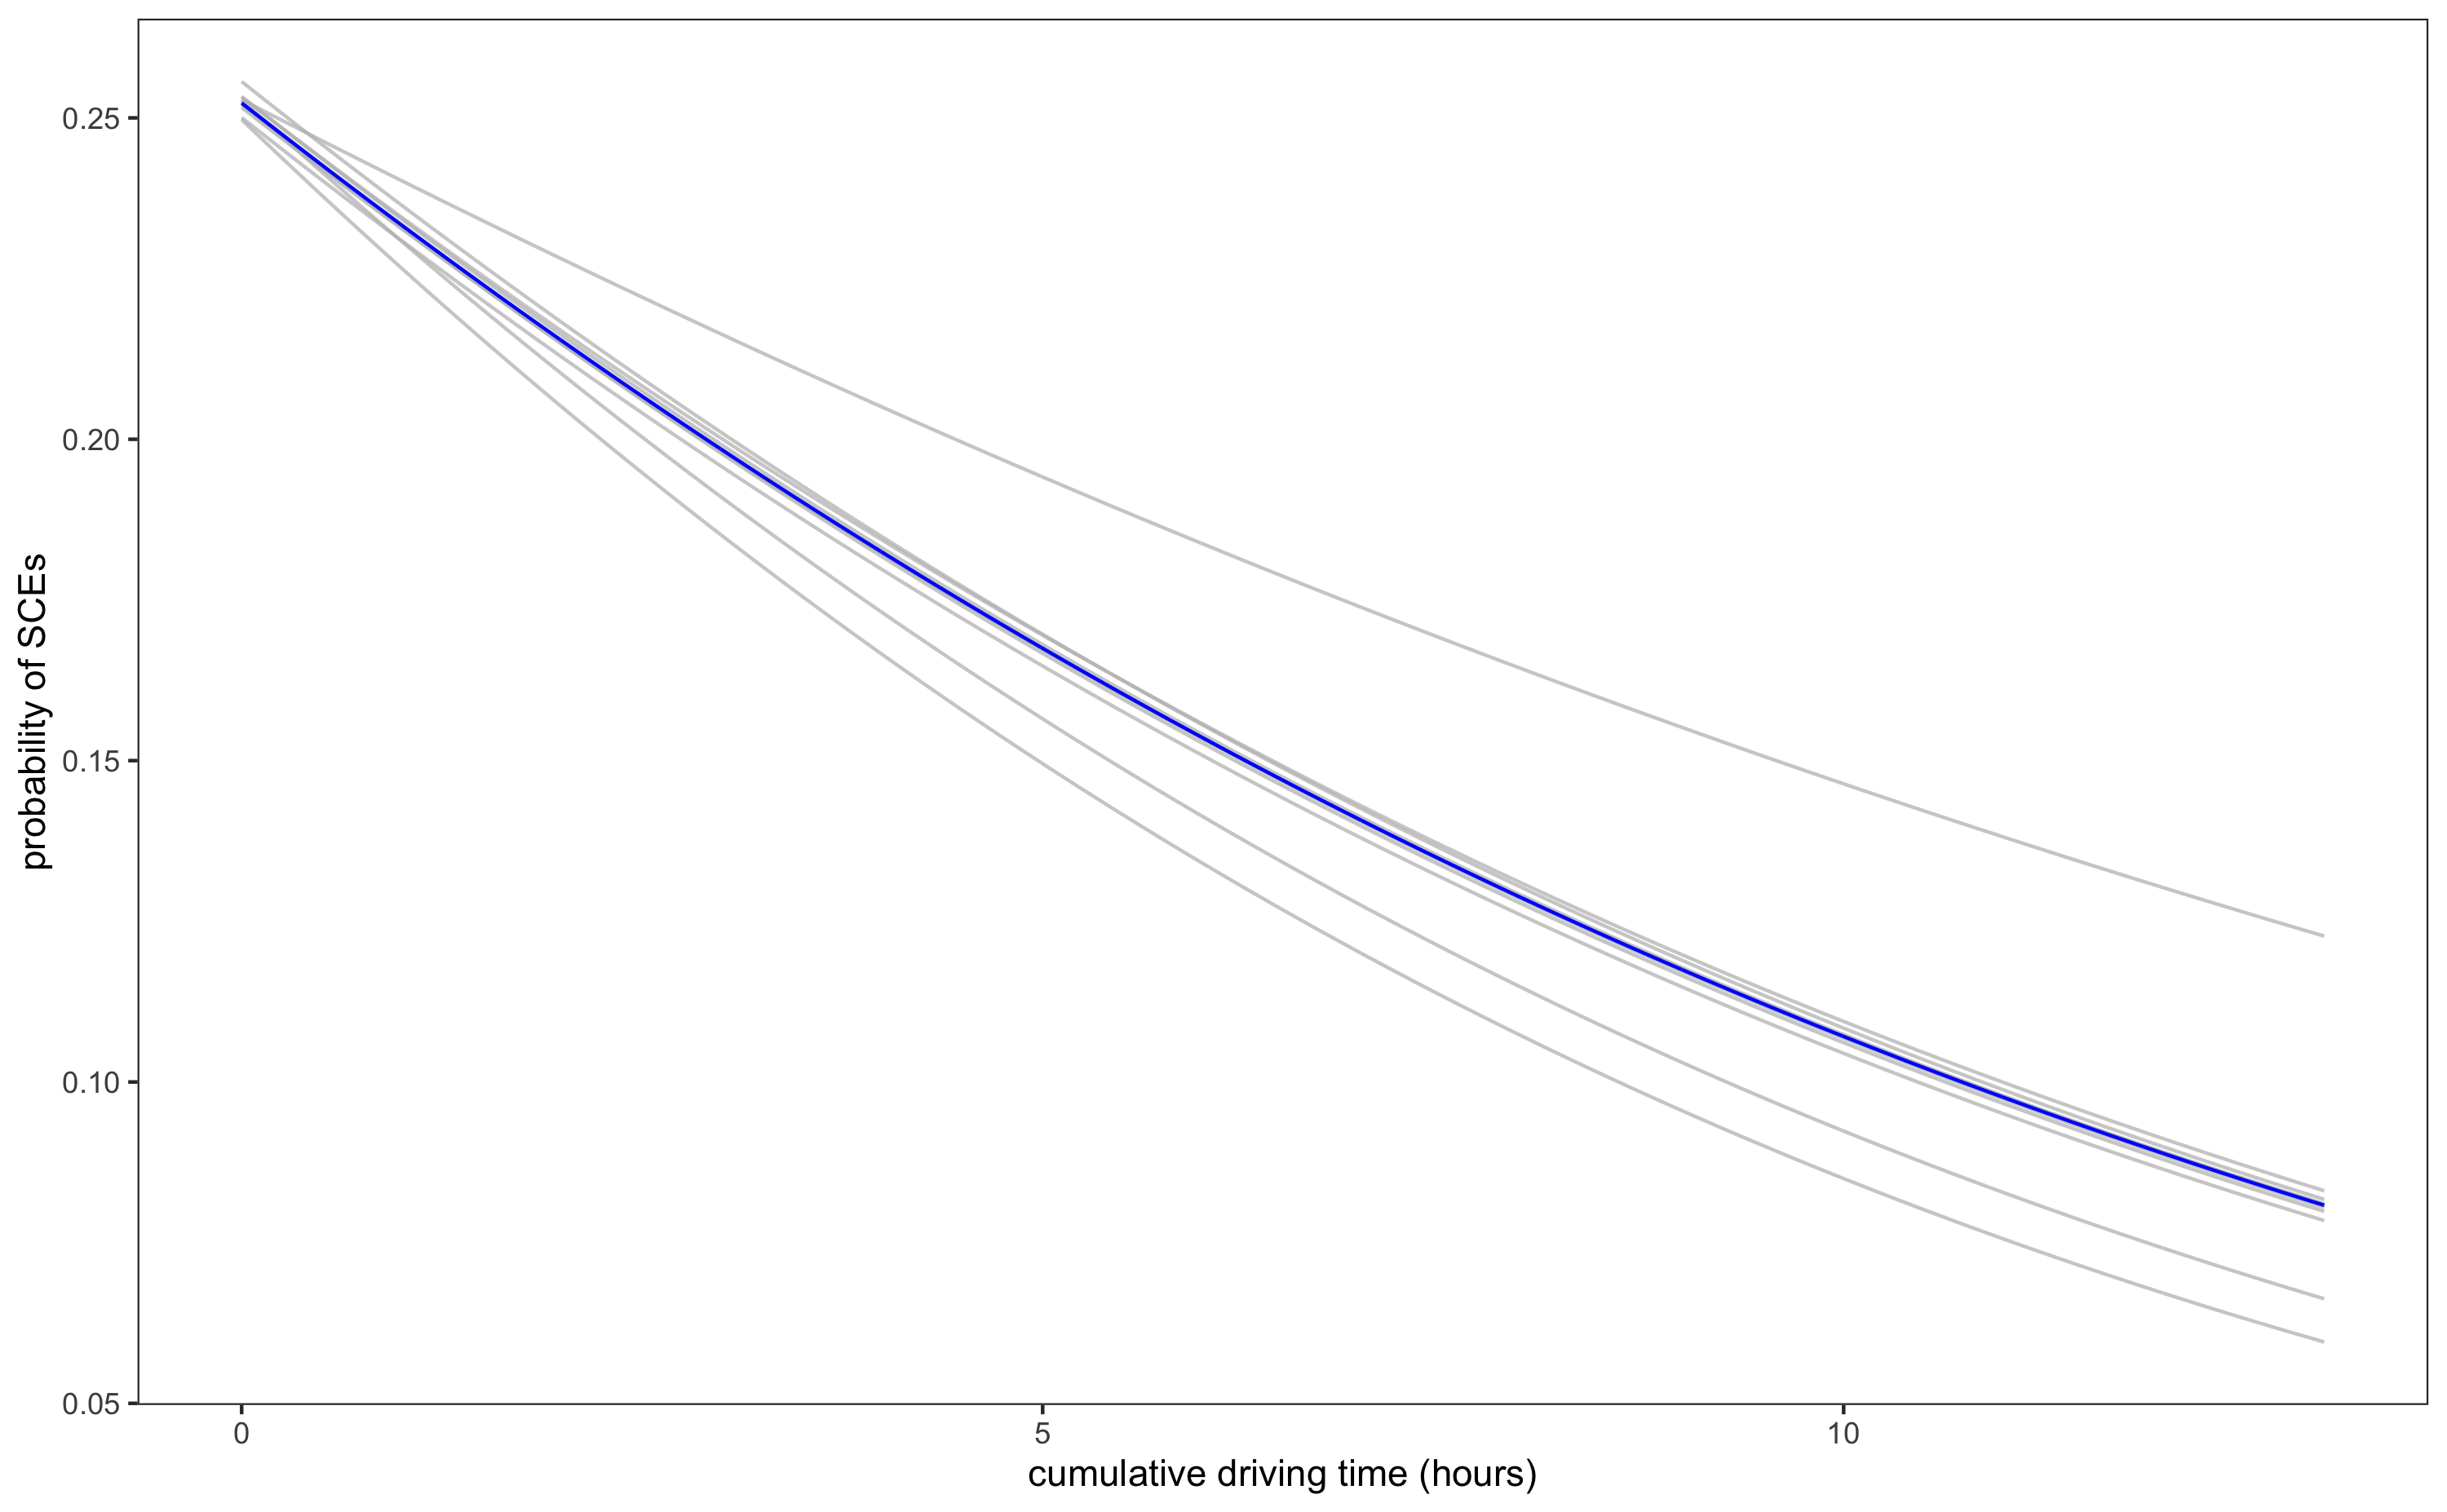
\includegraphics[width=\textwidth]{Figures/fit_logit.png}
  \caption{Cumulative driving time and estimated probability of SCEs from the hierarchical logistic model}
\end{figure}
\end{column}
\hfill
\begin{column}{.45\textwidth}
\begin{figure}
  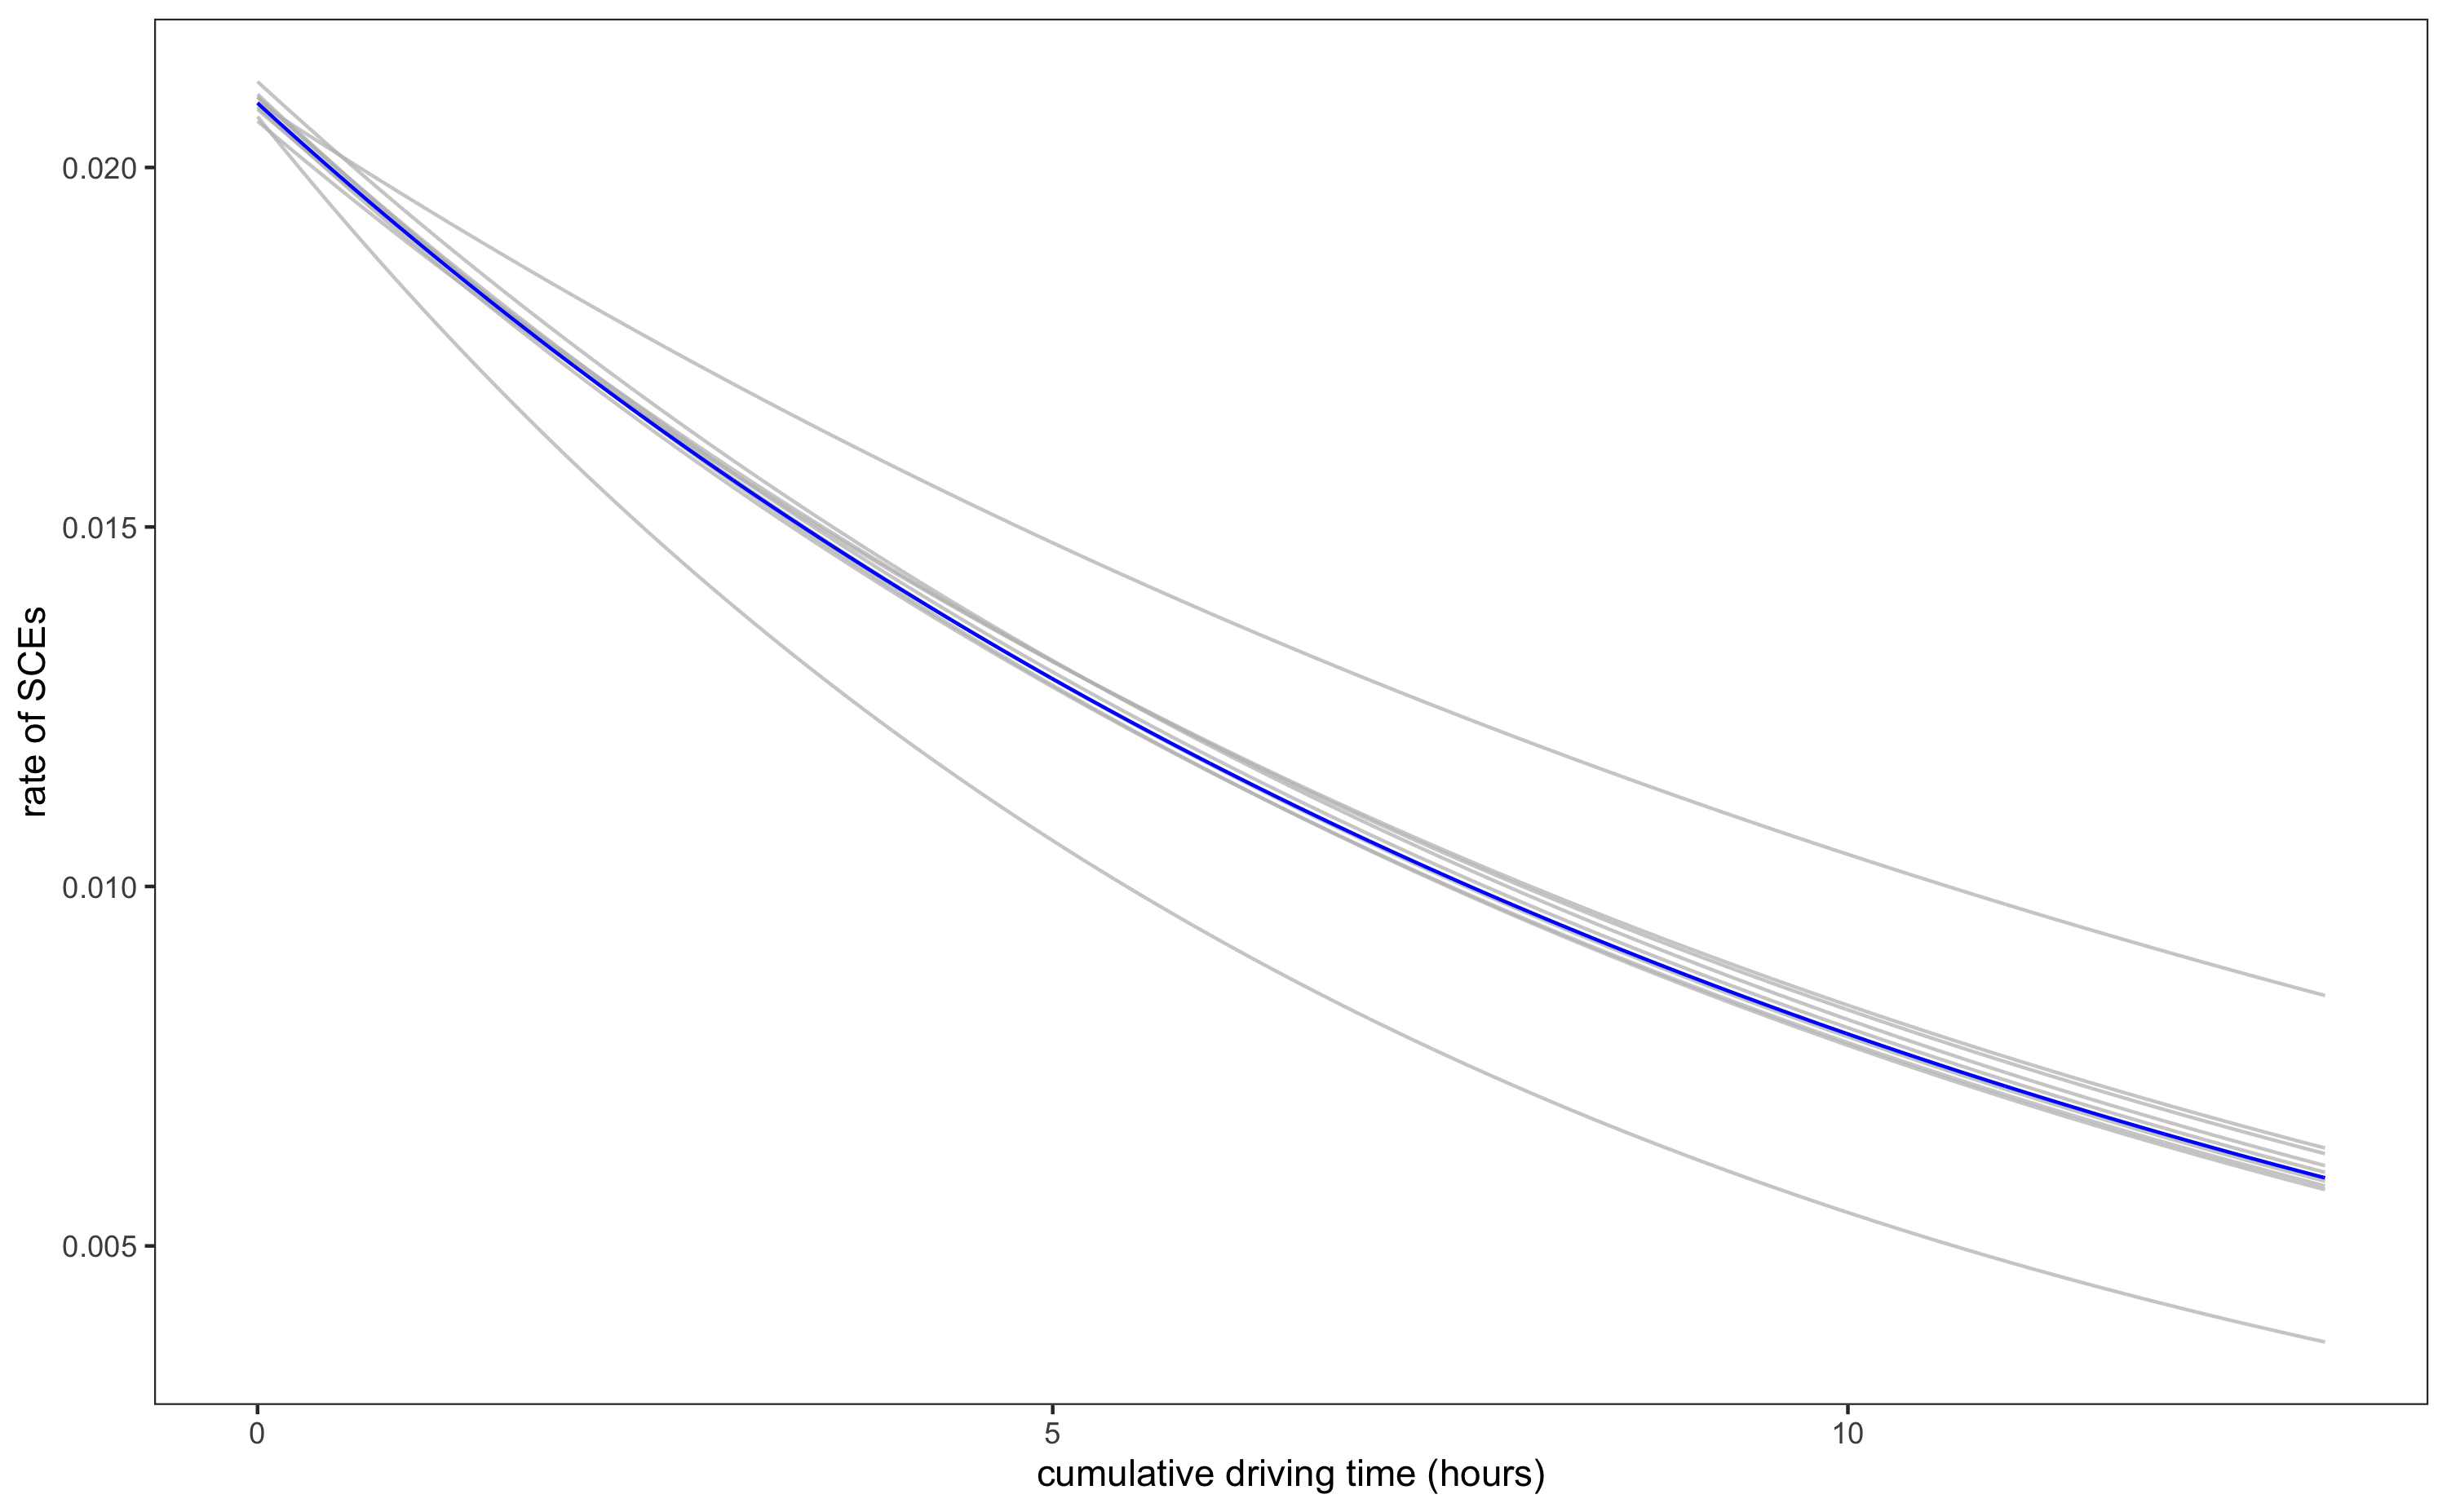
\includegraphics[width=\textwidth]{Figures/fit_Poisson.png}
  \caption{Cumulative driving time and estimated rate of SCEs from the hierarchical Poisson model}
\end{figure}
\end{column}
\end{columns}
\end{frame}

% Frame - results: NHPP
\begin{frame}{Results for hierarchical Bayesian NHPP}
\begin{figure}
  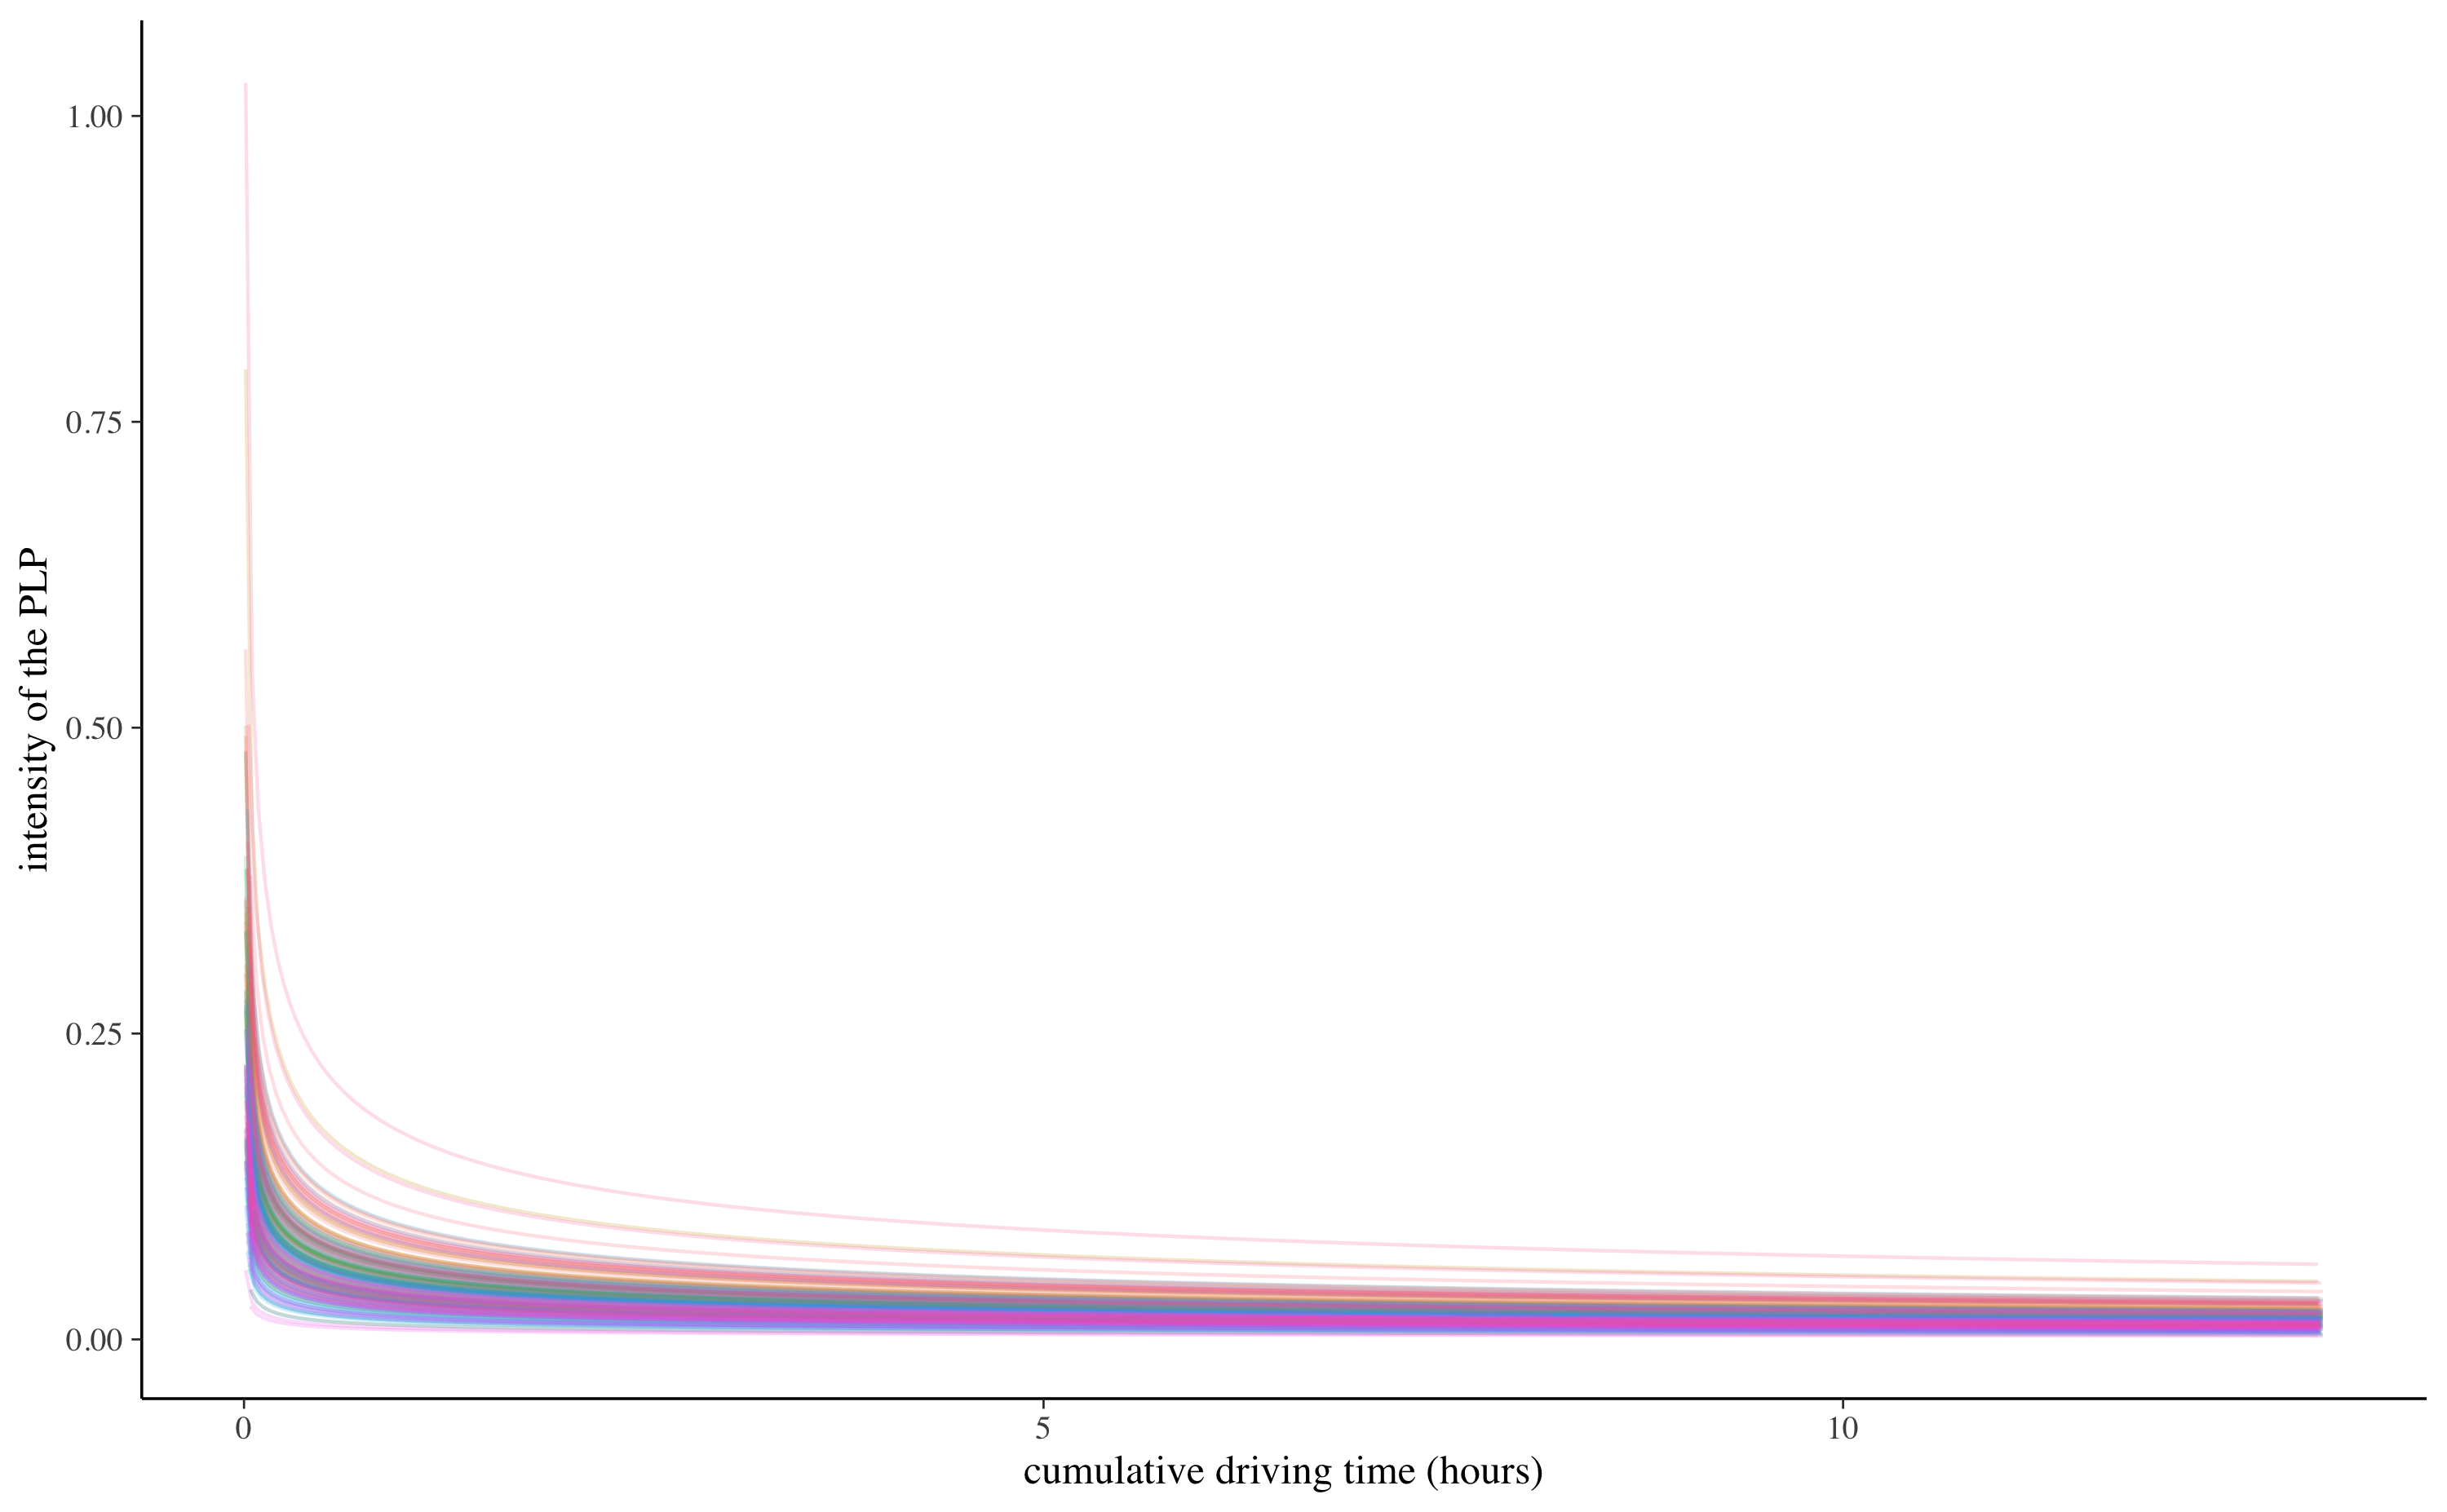
\includegraphics[height=0.45\textheight]{Figures/fit_plp.png}
  \caption{Cumulative driving time and estimated intensity of SCEs from the hierarchical NHPP.}
\end{figure}
\begin{itemize}
    \item 196 shifts for the 10 sample drivers,
    \item y-axis is the intensity of SCEs,
    \item Each line represents a shift, each color represents a driver.
\end{itemize}
\end{frame}